\documentclass{aion}

% Macros for Paper VII
\usepackage{eso-pic}
\usepackage{listings}
\usepackage{tabularx}
\usepackage{tikz}
\usetikzlibrary{arrows.meta,positioning,calc,fit,backgrounds}

\newcommand{\AION}{\textrm{AI}\ensuremath{\Omega}\textrm{N}}
\newcommand{\AIONProjectURL}{\url{https://github.com/flyingrobots/aion}}

% WARP term: small caps in prose, italic in math.
\DeclareRobustCommand{\WARP}{\ifmmode\mathit{WARP}\else{\upshape\scshape warp}\fi}

\newenvironment{argument}{\begin{proof}[Argument sketch]}{\end{proof}}

% Worked-example headings are authored as numbered subsections, but we keep their
% numbering stable and linkable as "Example 1/2/3" (independent of subsection
% numbering) so prose can cite "Example 3" directly.
\newcounter{workedexample}
\renewcommand{\theworkedexample}{\arabic{workedexample}}
\newcommand{\WorkedExample}[2]{%
  \refstepcounter{workedexample}%
  \subsection*{Example \theworkedexample: #1}%
  \phantomsection\label{#2}%
}
\newcommand{\Exref}[1]{\hyperref[#1]{Example~\ref*{#1}}}

\definecolor{AIONCodeBg}{RGB}{248,249,251}
\definecolor{AIONCodeRule}{RGB}{214,220,228}
\definecolor{AIONCodeString}{RGB}{130,48,20}
\definecolor{AIONCodeMeta}{RGB}{88,22,120}
\definecolor{AIONCodeKey}{RGB}{24,82,132}
\definecolor{AIONCodeComment}{RGB}{92,110,124}
\definecolor{AIONCodeNumber}{RGB}{120,126,138}
\definecolor{AIONTableStripe}{RGB}{246,247,249}
\definecolor{AIONTableHeader}{RGB}{236,239,243}

\newcommand{\AIONTableStyleOn}{%
  \rowcolors{2}{AIONTableStripe}{white}%
}
\newcommand{\AIONTableStyleOff}{%
  \relax
}
\newcommand{\AIONTableHead}{\rowcolor{AIONTableHeader}}

\lstdefinelanguage{AIONGraphQL}{
  sensitive=true,
  alsoletter={@,_},
  morecomment=[l]{\#},
  morestring=[b]",
  morekeywords=[1]{
    type,input,enum,interface,union,scalar,schema,directive,extend,on,
    implements,Mutation,Query,true,false,null
  },
  morekeywords=[2]{
    reads,writes,creates,slots,closures,createSlots,updates,forbids,
    slot,fromSlot,operator,argBindings,fields,bindFromArg,bindFromSlot,
    bindRelation,access,cardinality,kind
  },
  morekeywords=[3]{
    @wes_op,@wes_footprint,READ,WRITE,OPTIONAL,MANY
  }
}

\lstdefinestyle{aioncode}{
  language=AIONGraphQL,
  basicstyle=\ttfamily\small,
  keywordstyle=[1]\color{AIONBlue!85!black}\bfseries,
  keywordstyle=[2]\color{AIONCodeKey}\bfseries,
  keywordstyle=[3]\color{AIONCodeMeta}\bfseries,
  commentstyle=\color{AIONCodeComment}\itshape,
  stringstyle=\color{AIONCodeString},
  backgroundcolor=\color{AIONCodeBg},
  frame=single,
  rulecolor=\color{AIONCodeRule},
  framesep=6pt,
  framerule=0.6pt,
  numbers=left,
  numberstyle=\scriptsize\color{AIONCodeNumber},
  numbersep=10pt,
  stepnumber=1,
  firstnumber=1,
  xleftmargin=2.4em,
  xrightmargin=0.5em,
  breaklines=true,
  breakatwhitespace=false,
  columns=fullflexible,
  keepspaces=true,
  showstringspaces=false,
  aboveskip=0.8em,
  belowskip=0.8em
}

\tikzset{warp edge/.style={-{Latex[length=2.2mm,width=1.8mm]}, semithick}}
\tikzset{warp dashed/.style={warp edge, dashed}}
\tikzset{warp box/.style={draw=black, rounded corners=1.8pt, semithick, align=center, inner sep=4pt, fill=white, font=\small}}
\tikzset{warp stage/.style={warp box, fill=black!2}}
\tikzset{warp shell/.style={warp box, fill=black!4}}
\tikzset{warp small/.style={warp box, inner sep=3pt, font=\small}}
\tikzset{warp label/.style={font=\footnotesize, fill=white, inner sep=1.5pt, text=black!80}}
\tikzset{warp band/.style={draw=black!55, fill=black!5, rounded corners=6pt, line width=0.6pt}}
\tikzset{host node/.style={circle, draw=black, semithick, minimum size=8mm, inner sep=0pt, fill=white, font=\small}}
\tikzset{host edge/.style={draw=black, semithick}}
\tikzset{claim A/.style={draw=black!75, dashed, rounded corners=2pt, inner sep=4pt}}
\tikzset{claim B/.style={draw=black!65, densely dotted, rounded corners=2pt, inner sep=4pt}}
\tikzset{slice box/.style={draw=black!55, fill=black!6, rounded corners=2pt, inner sep=2pt}}

% Compatibility aliases for existing figures in the draft.
\tikzset{warpbox/.style={warp box}}
\tikzset{warpsmall/.style={warp small}}
\tikzset{warparrow/.style={warp edge}}
\tikzset{warpblocked/.style={warp dashed}}
\tikzset{warplabel/.style={warp label}}
\tikzset{warpghost/.style={warp box, dashed, fill=white}}
\tikzset{hostnode/.style={host node}}
\tikzset{hostedge/.style={host edge}}
\tikzset{matchboxA/.style={claim A}}
\tikzset{matchboxB/.style={claim B}}

\newcommand{\AIONDraftWatermark}{%
  \AddToShipoutPictureBG{%
    \AtPageLowerLeft{%
      \raisebox{0.18\paperheight}[0pt][0pt]{%
        \hspace*{0.16in}%
        \rotatebox{90}{%
          \textcolor{AIONAccent!35}{\fontsize{18}{22}\selectfont\bfseries ROUGH DRAFT \quad ROUGH DRAFT \quad ROUGH DRAFT}%
        }%
      }%
    }%
  }%
}


% We use a small number of non-floating figures to keep worked examples adjacent
% to their explanatory text.
\usepackage{float}
\usepackage{needspace}

% Use global figure numbering (Figure 1, 2, 3, ...) rather than per-section
% numbering. Paper VII reads better with a single figure sequence.
\counterwithout{figure}{section}
\renewcommand{\theHfigure}{\arabic{figure}}

% ------------------------------------------------------------
% Metadata for this paper
% ------------------------------------------------------------
\renewcommand{\papertitle}{WARP: Optics, Holograms, and Worldlines over Shared Causal History}
\renewcommand{\papernumber}{Paper VII}
\renewcommand{\paperdate}{April 2026}

\renewcommand{\paperauthor}{James Ross}
\renewcommand{\paperaffiliation}{Independent Researcher}
\renewcommand{\paperorcid}{0009-0006-0025-7801}
\renewcommand{\paperdoi}{10.5281/zenodo.19751149}
\renewcommand{\papercopyrightyear}{2026}

% Embed publication metadata in the PDF itself (not just the visible title page).
\hypersetup{
	pdftitle={\papertitle},
	pdfauthor={\paperauthor},
	pdfsubject={AION Foundations Paper VII},
	pdfkeywords={AION Foundations, WARP, optics, holograms, worldlines, causal history, deterministic replay, provenance, distributed systems},
}

\begin{document}

% Draft watermark (disabled for release builds).
%\AIONDraftWatermark

\AIONFrontMatter{
		We define \WARP{} as an optic architecture over shared causal history. A \WARP{}
		optic places an observer-relative aperture over a bounded slice of causal
		history, lowers the resulting weave under an admissibility law, and retains a
		holographic witness sufficient for replay, audit, transport, and bounded
		revelation. Deterministic ticks, braid collapse, and replica import are thus
		instances of one recurring act: slice, lower, witness, retain.

		We argue that \WARP{} is closed over its own witness-bearing outputs. A tick
		receipt, braid shell, import shell, or property certificate is itself a
		first-class object for later folding, revelation, comparison, or reliance,
		not an after-the-fact log attached to an execution.

		The distributed consequence is direct: network distance does not introduce a
		second admission law. Transport constructs the comparable slice on which
		replica-scale lowering can occur; once that slice exists, the downstream optic
		is the same one already used locally. Distribution changes the slice boundary;
		it does not change the downstream law.
}

\section{Introduction}

The preceding \AION{} papers \cite{Ross2025I,Ross2025II,Ross2025III,Ross2025IV,Ross2026V,Ross2026VI}
established the mechanisms that make \WARP{} distinctive: deterministic execution,
provenance-complete boundary artefacts, observer-relative revelation, executable
branching over shared prefixes, and the sovereignty pressure created by replayable
shared history. This paper does not add another mechanism. It names the control
shape that makes those mechanisms one architecture. That object is the \WARP{} optic
(Definition~3.1).

The optic is a composite act. It begins with a positioned observer and a weave of
plural claims, constructs a bounded slice on which judgement is lawful, admits a
witnessed outcome under policy, and retains a holographic boundary for later replay,
audit, transport, or bounded revelation (Section~3). The same act recurs at tick,
braid, and replica scale (Section~4), and we ground each scale in a worked example
(Section~5).

We use a direct noun map and then enforce it. A worldline carries admitted causal
history. A weave holds basis-relative claims in suspension. An optic lowers that weave
through a bounded aperture under policy. A hologram retains the witness-bearing
boundary of the lowering. These nouns are not synonyms for older rewrite vocabulary;
they separate responsibilities that otherwise blur together in implementation: basis
construction, lawful judgement, and retained obligations.

We also state one ontology choice early, because it stabilises the rest of the paper.
We treat witnessed causal history as primary: admitted transitions, frontiers, witnesses,
and retained boundary artefacts are the primitive objects. ``The graph'' then names a
frontier-relative chart over that history, emitted by an observer under a lawful basis
and aperture. This makes \WARP{} graph-expressive without committing the architecture
to a privileged materialised graph object underneath it.

Two consequences are derived and then reused throughout. First, \WARP{} is closed over
its own witness-bearing outputs (Proposition \emph{Closure over witness-bearing outputs} in
Section~3): receipts, braid shells, import shells, and certificates are first-class objects
for later folding, revelation, comparison, or certification. Secondly, distribution changes
what must be normalised to become comparable before judgement; it does not introduce a
second admission law (Section~4 and Example~5.3).

Reducer or rewrite language explains a local transformation. The optic form explains the
larger control law around that transformation: bounded focus, lawful judgement, retained
residual, and reuse across execution, replay, explanation, transport, and revelation. It is
also the reason we adopt the profunctor form in Section~3.1: the same declared optic should
support multiple interpretations without changing its structural focus.

\paragraph{Position in the series and neighbouring work.}
This paper extracts the invariant the earlier foundations papers approached in part. The present discussion therefore sits at the intersection of algebraic graph transformation \cite{Ehrig2006,Corradini1997}, event structures and causal partial orders \cite{Lamport1978,Winskel1987}, process semantics \cite{Hoare1985,Milner1989,Park1981}, provenance systems \cite{Buneman2001,Cheney2009}, and distributed reconciliation \cite{DeCandia2007,Shapiro2011,GilbertLynch2002}. Its contribution is the identification of the optic-shaped law that recurs across them and the architectural consequences of taking that law seriously.

\paragraph{Contributions.}
The specific contributions are:

\begin{enumerate}[leftmargin=*]
	\item An optic-centered reframing of \WARP{} around four primary nouns: worldlines, weaves, optics, and holograms.

	\item A native definition of the \WARP{} optic, separating observer structure, bounded aperture, set-side lowering, admissibility law, and retention contract.

	\item A clarification of why the optic form matters: the same declared \WARP{} act may lawfully support execution, footprint derivation, witness extraction, debugger explanation, translation analysis, and schema compilation---that is, compilation of app-authored optic surfaces into runtime-checkable intent and observer artefacts---without changing its structural focus.

	\item A scale-by-scale identification of the same optic-shaped lowering in three primary settings: local tick execution, braid-local collapse, and distributed suffix import after transport to a common basis.

	\item A recursive hologram result: each such lowering emits a boundary-complete shell for the bounded admitted situation, so replay, audit, transport, and counterfactual examination propagate beyond ticks to braid-local, replica-local, and later trust-bearing shells.

	\item A normalisation thesis for distributed causality: network distance relocates the hard part into transport and normalisation to a comparable frontier.

	\item A three-way architectural decomposition into commitment, folding, and revelation, separating what is true from how it is stored and who may lawfully inspect it.

	\item A post-Unix reframing in which processes and files are treated as materialised views over shared causal history, together with a protected working interval spanning ephemeral, author-only, and shared lanes.

	\item An architectural bridge from provenance to privacy through property certificates, reliance status, and observer rights, showing how bounded revelation can coexist with replayable history.
\end{enumerate}

\paragraph{Scope.}
This paper is architectural, with a small amount of formal structure. Its goal is to extract the common optic shape that recurs across the \WARP{} stack and to show how that shape supports both strong provenance and bounded revelation. The remaining frontier laws opened by this view---including contamination calculus, collective sovereignty, export semantics, and hostile transport conditions---remain follow-on work. The present paper fixes the architectural centre with sufficient precision that those later laws can be treated as extensions. Accordingly, most formal statements in this paper are propositions with argument sketches about recurrent structure; only the replica-scale confluence result is stated as a theorem because it makes a specific behavioural claim about retained shells.

\paragraph{Reading guide.}
Section~2 stabilises the noun map. Section~3 gives the core optic definition and
the local laws needed to read it. Section~4 then states the recurrent
scale-local claims. The remaining sections draw distributed, systems, and
governance consequences from that control shape.

\clearpage
\section{Causal Lanes, Strands, and Braids}

Before defining the optic, we need the basic ontology. The earlier papers developed deterministic execution, branching, and replay, but they did not need to stabilise the noun map at this level of explicitness. Here we do, because the same optic acts over different kinds of objects, and those objects must not be allowed to collapse into one another.

\begin{definition}[Causal lane]
	A \emph{causal lane} is a replayable carrier of causal history equipped with a
	frontier-relative materialisation map. At minimum, a lane has an identity, an
	event or tick order, a causal provenance record, and a rule by which a frontier
	or tick determines a materialised state.
\end{definition}

This use of lanes is intentionally close to the older language of events, causal
dependence, and partial orders: it assumes that a computation admits multiple
serialisations, with its causal structure captured by partial orders
\cite{Lamport1978,Winskel1987}.

The term \emph{lane} is therefore the ontology-level noun for a history-bearing computational object. It is intentionally broader than \emph{worldline}. A lane may be canonical or speculative; it may already be socially admitted, or it may still be a private counterfactual carrier.

\begin{definition}[Worldline]
	A \emph{worldline} is a canonically admitted causal lane. It is the lane form whose history and frontier-relative materialisations count as shared causal reality for the relevant policy frame.
\end{definition}

\begin{definition}[Strand]
	A \emph{strand} is a speculative causal lane rooted at a parent worldline and a fork anchor. A strand carries fork provenance back to that parent anchor, together with whatever local history is required for the strand to diverge lawfully from the inherited base.
\end{definition}

Two consequences should be kept explicit. First, a strand is a real lane with causal identity and fork provenance. Secondly, its definition is a divergence record that can be resolved at multiple bases. Its materialisation at a given frontier is obtained by resolving the strand's local divergence against the inherited parent history at the chosen basis.

Operationally, this means a strand is read holographically. A bounded read of a
strand materialises only the backward causal cone required by the strand's local
divergence and optic footprint at the chosen basis. The strand is real as a
speculative lane; its realised state is a frontier-relative reading over
inherited history plus local divergence, and it avoids eager copying of the
whole parent lane.

\begin{definition}[Braid]
		A \emph{braid} is a lane-scale weave: a plural composition over a family of lanes sharing a common precursor or comparison basis. It presents multiple validated lane claims over a common frontier so that a later collapse or admission act may judge them.
\end{definition}

\begin{definition}[Weave]
	A \emph{weave} is a basis-relative carrier that holds multiple candidate claims in suspension without yet forcing a single derived answer. Candidate rewrite bundles, braids, and transported import families are the three primary weaves studied in this paper.
\end{definition}

The name is geometric: we use ``braid'' because lane traces literally interweave over a shared basis. Full braid-group machinery is outside the present scope \cite{Artin1947}. This is also the first place where ordinary version-control language becomes misleading. A braid is not a latent merge result. It is the weave over which collapse may later derive a lane-level result, preserve plurality, surface conflict, or return obstruction. In that respect it is closer to patch-theoretic comparison objects than to a preordained merge target \cite{MimramDiGiusto2013}.

\begin{remark}[Ontology versus realisation]
		These nouns are ontology-level nouns. Realisation-level objects are
		frontier-relative views: a strand resolved at a particular parent frontier,
		or a braid presented over a specific common basis. This distinction is
		necessary because a strand may be a stable noun while its realised view
		changes with the frontier at which it is interpreted.
\end{remark}

The same split also prevents admission from silently doing other jobs. Forking creates ancestry. Braiding constructs a weave. Collapse derives a lane-level result from that weave when policy and witness conditions allow it. Admission, finally, blesses a derived result as canonical when the governing law requires that further step. If these verbs are allowed to blur together, the rest of the paper becomes incoherent.

\paragraph{Operational intuition.}
A worldline is the shared lane others may rely on. A strand is the speculative lane in which counterfactual or author-local work may proceed without immediately becoming shared fact. A braid is the object that appears when several such lanes must be compared over one basis without yet pretending they have collapsed into a single answer. The optic introduced next acts over all three scales, but it acts over a different weave at each scale.

% Keep the specification note and terminology summary from being split by a page
% break, but avoid pushing the entire block onto a fresh page and leaving an
% awkward blank region.
\Needspace{10\baselineskip}
\paragraph{Specification note.}
We keep the runtime interface out of line. The noun map is
implementation-bearing, but the concrete interface depends on the host language
and toolchain. In the current stack, authored SDL boundaries are compiled by
a schema compiler into generated host bindings and runtime-checkable footprint,
witness, and retention obligations. The present paper fixes the invariant
control shape that those compilations implement.

\paragraph{Terminology summary.}
\begin{center}
	\small
	\setlength{\tabcolsep}{4pt}
	\renewcommand{\arraystretch}{1.05}
	\begin{tabularx}{\textwidth}{@{}>{\raggedright\arraybackslash}p{0.18\textwidth}X>{\raggedright\arraybackslash}p{0.30\textwidth}@{}}
		\toprule
		Terminology & Definition & Remarks \\
		\midrule
		Causal lane & Replayable carrier of causal history with frontier-relative materialisation. & May be canonical or speculative. \\
		Worldline   & Canonically admitted causal lane. & Counts as shared causal reality under the governing policy frame. \\
		Strand      & Speculative causal lane rooted at a parent worldline and fork anchor. & Resolves divergence against a chosen basis. \\
		Braid       & Lane-scale weave over multiple lanes sharing a common precursor or basis. & Comparison carrier presented for later collapse or admission. \\
		Weave       & Basis-relative carrier of suspended candidate claims. & Tick bundles, braids, and transported import families are the primary cases. \\
		Hologram    & Retained boundary sufficient to recover the optic-accurate bulk under a retention contract. & Shell \(\theta\) is a concrete carrier of a hologram. \\
		\bottomrule
	\end{tabularx}
\end{center}

\clearpage
\section{The WARP Optic}

Our main object is the \WARP{} optic. It names the composite act from which
local execution, braid collapse, replica import, replay, debugger explanation,
and witness retention are all built. A \WARP{} optic couples a positioned
observer to a bounded site, a lawful set-side lowering, and the retained
boundary that later makes that act replayable, auditable, transportable, or
revealable.

\begin{definition}[WARP optic]
	Fix an observer plan \(\Omega = (\pi,\beta,M,U,E)\). A
	\emph{\WARP{} optic} is a tuple
	\[
		\Psi = (\Omega,\chi,\rho,\Pi,\Lambda)
	\]
	where:
	\begin{itemize}[leftmargin=*]
		\item \(\Omega\) fixes the revelation-side observer discipline: projection,
		      basis, observer state, update discipline, and emission;
		\item \(\chi\) is the bounded aperture or optic slice within which a local
		      judgement is lawful;
		\item \(\rho\) is the set-side lowering surface that presents a comparable
		      claim surface over \(\chi\) from a frontier-relative weave;
		\item \(\Pi\) is the admissibility law governing what may be derived,
		      preserved as plural, surfaced as conflict, or obstructed at that slice;
		\item \(\Lambda\) is the retention contract specifying which replay, audit,
		      transport, revelation, or reliance obligations the retained shell must still
		      satisfy.
	\end{itemize}
\end{definition}

A \WARP{} optic acts on a basis-relative weave
\(\mathcal{P}\). We write
\[
	\operatorname{Lower}_{\Psi}(F_*, \mathcal{P}) = (R,W,\theta)
\]
with the internal factorisation
\[
	(C,\chi) = \rho(F_*, \mathcal{P}; \Omega),
	\qquad
	(R,W) = \operatorname{Admit}_{\Pi}(F_*, C, \chi),
	\qquad
	\theta = \operatorname{Pack}_{\Lambda}(R, W).
\]
The internal names remain useful. We treat the optic as the primary object,
with these helper acts serving as its internal factorisation.

Lowering names the composite optic act. Admission names the policy judgement
inside that act. \WARP{} therefore remains an admission architecture: the
optic first constructs a comparable slice, then admits, preserves plurality,
surfaces conflict, or obstructs under policy, and finally packs the witnessed
outcome into a retained shell.

\paragraph{Tiny worked instance.}
At tick scale, one can read the factorisation almost literally. Let
\(\mathcal{P}=\{c_1,c_2\}\) be two candidate rewrites whose footprint overlaps at
a node \(n\). Then \(\rho\) presents the local claim surface over the footprint
slice \(\chi=\mathrm{footprint}(n)\), admission returns a derived outcome plus a
witness of the blocked coexistence, and packing retains a receipt-like shell:
\[
	(C,\chi) = \rho(F_*, \{c_1,c_2\};\Omega),
	\quad
	(R,W)=\operatorname{Admit}_{\Pi}(F_*,C,\chi),
	\quad
	\theta=\operatorname{Pack}_{\Lambda}(R,W).
\]
The point is not the toy \(n\), but the separation of responsibilities: basis
construction, lawful judgement, then retention.

This presentation also keeps the set side architectural. One runtime may
realise \(\rho\) by bounded DPO graph rewriting; another may realise it by
CRDT-style set semantics over an append-only history. We name the invariant
role and leave the specific calculus open.

\paragraph{Three immediate specialisations.}
The definition is intentionally generic, but it should already read
concretely in the three primary cases:
\begin{itemize}[leftmargin=*]
	\item at tick scale, \(\mathcal{P}=C_{\mathrm{rw}}\) is the candidate rewrite
	      bundle and \(\rho\) returns the local footprint slice over one current
	      frontier;
	\item at braid scale, \(\mathcal{P}=B\) is the braid and \(\rho\) returns the
	      common-basis comparison slice over the participating strands;
	\item at replica scale, \(\mathcal{P}=\widetilde{C}\) is the transported
	      remote suffix family and \(\rho\) returns the imported-region slice at the
	      receiver's comparable frontier.
\end{itemize}
The optic law is the same in all three cases. What changes is the weave and the
work needed to present a comparable slice for lawful judgement.

\begin{definition}[Optic slice]
	The bounded site \(\chi\) is the \emph{optic slice}: the least
	frontier-relative closure over which the governing law can lawfully compare the
	claims in the weave and judge their coexistence, derivation, plurality, conflict, or
	obstruction. The lowering surface produces claims over such a slice; the
	hologram later preserves the result slice needed for replay, audit, transport,
	or revelation. This generalises the spirit of program slicing---isolating what
	is relevant to a criterion---from program statements to witnessed causal
	history \cite{Weiser1981}.
\end{definition}

We make the outcome space explicit with one typing. Let \(X\) be the
scale-local carrier of derived results. Then
\[
	\mathcal{O}(X)
	:=
	\operatorname{Derived}(X)
	\;\sqcup\;
	\operatorname{Plural}(X)
	\;\sqcup\;
	\operatorname{Conflict}
	\;\sqcup\;
	\operatorname{Obstruction}.
\]
Optic lowering returns a witnessed member of an outcome algebra.

Truth should be read operationally here. In \WARP{}, ``truth'' names what may be
lawfully admitted relative to a frontier, an optic, and a witness. Lowering
therefore supports more than binary accept or reject: lawful outcomes may also
preserve plurality, surface conflict, or return obstruction.

\subsection{Why The Optic Form Matters}

The optic form matters because the same declared optic should support more than
one interpretation. In profunctor form,
\(\mathsf{Opt} : p\,a\,b \to p\,s\,t\),
varying the profunctor \(p\) changes how the act is interpreted while leaving
its structural focus unchanged. For \WARP{}, we use this to reuse one declared
optic for execution, footprint and slice derivation, witness extraction or
validation, debugger explanation, translation analysis, and compilation.

The term \emph{optic} is used in deliberate continuity with the lens and
profunctor-optics tradition, in which a focused transformation can be lifted
into a transformation of a larger whole \cite{Foster2007,Pickering2017,Boisseau2018}. \WARP{}
uses the optic discipline architecturally. We separate focus and residual from
lawful judgement, witness, and observer-relative emission, so that execution,
replay, explanation, and revelation can share one declared structure.

In profunctor notation, the core optic idea is:
\[
	\mathsf{Opt} : p\,a\,b \to p\,s\,t
\]
where \(s\) and \(t\) are the whole before and after the act, \(a\) and \(b\)
are the focused part before and after the act, and \(p\) is an abstract
transformation context. Read operationally: if one can transform the focused
part from \(a\) to \(b\) inside some lawful context \(p\), the optic lifts that
into a transformation of the whole from \(s\) to \(t\).

For \WARP{}, the important consequence is that the same declared optic can be
interpreted multiple ways without changing its structural focus. The same act
may therefore be reused to:
\begin{itemize}[leftmargin=*]
	\item execute the local lowering,
	\item derive the optic slice or footprint,
	\item derive or validate the witness,
	\item render a debugger explanation,
	\item estimate conflict or translation cost,
	\item or emit a compiler-produced runtime artefact.
\end{itemize}
That reuse is one of the main reasons the paper needs optic language in addition
to reducer language.

\subsection{Residual, Witness, and Hologram}

The optic story includes a hidden residual. For a lens-like optic, one standard
representation is \cite{Pickering2017,Boisseau2018}
\[
	\mathrm{Lens}(S,T,A,B)
	\cong
	\int^{M}
	\mathcal{C}(S, M \times A)
	\times
	\mathcal{C}(M \times B, T).
\]
This says that the whole \(S\) can be decomposed into a focused part \(A\) and
a hidden residual \(M\), then reassembled from the updated focus \(B\) and
that same residual. The coend matters because the optic semantics does not care
about one privileged presentation of the residual. It quotients over
equivalent presentations of the hidden context.

That perspective is exactly the right intuition for \WARP{} shell equivalence.
Two retained shells may preserve the same optic-accurate bulk of a bounded
admitted situation while differing in their concrete storage shape. The witness
\(W\) is the residue explaining why the lowering was lawful; in the constructive
tradition, it is closer to a proof-bearing object than to an after-the-fact
annotation \cite{MartinLof1984}. The hologram \(\theta\) is the retained carrier.
A Boundary Transition Record is therefore not the optic law itself. It is one
concrete shell family carrying the law's consequences for later use.

In lens language the residual \(M\) is typically hidden. In \WARP{}, the
residual is made explicit and split: \(\theta\) is the retained carrier, \(W\)
is the witness-bearing residue explaining lawfulness, and \(\Lambda\) names the
future obligations that equivalence must preserve.

	\begin{definition}[Optic-accurate bulk]
		For optic \(\Psi\) and retention contract \(\Lambda\), the
		\emph{optic-accurate bulk} of a bounded admitted situation is the portion of
		that situation, together with the witness structure it requires, that must
		remain recoverable for the lawful observations and obligations named by
		\(\Psi\) and \(\Lambda\). It is a bounded notion: the retained causal content
		sufficient for the replay, audit, transport, revelation, or reliance uses
		permitted at that aperture.
	\end{definition}

\begin{definition}[WARP hologram]
	For optic \(\Psi\) and lowering result
	\[
		\operatorname{Lower}_{\Psi}(F_*, \mathcal{P}) = (R,W,\theta),
	\]
		a \emph{\WARP{} hologram} is the retained shell \(\theta\), together with any
		referenced basis anchors, such that \(\theta\) is sufficient to recover the
		optic-accurate bulk of the bounded admitted situation, as determined by
		\(\Psi\), up to the equivalence demanded by the retention contract
		\(\Lambda\). The contract is explicit: preserve the least sufficient boundary
		from which the admitted outcome and its witness-bearing consequences can be
		reconstructed, replayed, audited, transported, or revealed as \(\Lambda\)
		requires.
	\end{definition}

\begin{proposition}[Closure over witness-bearing outputs]
	\WARP{} is closed over its own witness-bearing outputs. For each primary scale
	\(s \in \{\mathrm{tick}, \mathrm{braid}, \mathrm{replica}\}\), there exists a
	scale-local optic \(\Psi_s\) and a scale-local weave
	\(\mathcal{P}_s\) such that
	\[
		\operatorname{Lower}_{\Psi_s}(F_s, \mathcal{P}_s)
		=
		(R_s,W_s,\theta_s),
	\]
	and the resulting hologram \(\theta_s\) is itself a first-class object of
	later folding, revelation, certification, or further lawful comparison.
\end{proposition}

\begin{argument}
	At tick scale, the weave is the local candidate rewrite
	bundle; the hologram preserves the frontier coordinate, the admitted result,
	and the witness explaining coexistence or blockage for one lawful step. At
		braid scale, the weave is the braid over a common basis; the
		hologram preserves the bounded comparison geometry and the lawful collapse or
		plural outcome. At replica scale, the weave is the remote
		suffix family as re-expressed at a comparable frontier; the hologram preserves
		the imported region, the import outcome, and the transport/import witness. In
		each case the retained shell is a first-class \WARP{} object, so later lawful
		acts can operate over it without leaving the ontology of witnessed causal
		history.
	\end{argument}

	This closure is what makes the architecture self-similar across scale. A local
	tick receipt, a braid-collapse artefact, a transport/import shell, and a trust
	certificate are members of one shell family: retained holographic boundaries
	over bounded admitted situations. Because each recurrence emits such a
	hologram, deterministic replay and counterfactual examination recur with the
	law itself. Each retained slice stores the least sufficient history of its
	bounded local situation.

\subsection{Commitment, Folding, Revelation}

The optic architecture becomes easier to navigate once the stack is divided
into three moments:

\begin{itemize}[leftmargin=*]
	\item \textbf{Commitment}: a weave is lowered into
	      frontier-relative truth under a governing optic.
	\item \textbf{Folding}: already-admitted history is re-expressed in a
	      boundary-equivalent retained shell.
	\item \textbf{Revelation}: admitted or folded history is exposed to a bounded
	      observer under an aperture and authority regime.
\end{itemize}

	This three-way split is one of the main architectural results. It
	keeps the system from conflating what is true, how truth is stored, and who may
	see it.
	Commitment records the witnessed outcome of lawful judgement: derivation,
	preserved plurality, conflict, or obstruction.

	The equivalence relation is intentionally behavioural: it preserves the
	lawful observations and replay obligations promised by a retained contract. In
	that sense it is closer to bisimulation and observational equivalence than to
	storage equality \cite{Park1981,Milner1989}.

\begin{definition}[Shell equivalence]
	Let \(\Lambda\) be a retained contract specifying which replay, audit,
	transport, or revelation obligations must remain lawful. Two shells
	\(\theta\) and \(\theta'\) satisfy
	\[
		\theta \simeq_{\Lambda} \theta'
	\]
	iff they are both sufficient to recover the same optic-accurate bulk of the
	same admitted local situation for the lawful uses demanded by \(\Lambda\).
\end{definition}

We give one small example. A tick receipt that stores an inverse fragment inline
and a folded shell that stores only digest-plus-pointer references may still be
\(\Lambda\)-equivalent for replay and audit if both reconstruct the same local
rewrite, witness anchors, and retained obligations. They cease to be equivalent
once \(\Lambda\) demands a lawful use---for example immediate plaintext
revelation---that only one of them can satisfy.

For later use, the three moments can be written as typed acts:
\[
	\operatorname{Commit}_{\Psi}(F_*, \mathcal{P})
	:=
	(R,W,\theta)
\]
where
\[
	(R,W,\theta) = \operatorname{Lower}_{\Psi}(F_*, \mathcal{P}).
\]

\[
	\operatorname{Fold}_{\Lambda}(\theta) = \theta'
	\qquad
	\text{with}
	\qquad
	\theta' \simeq_{\Lambda} \theta.
\]

\[
	\operatorname{Reveal}_{\Omega,\alpha}(m,\theta)
	=
	(m', y, W_{\mathrm{rev}})
\]
where \(\Omega = (\pi,\beta,M,U,E)\) is an observer plan, \(\alpha\) is
the active authority regime, \(m \in M\) is the current observer state, and
\(y\) is the emitted reading. The observer plan is the revelation-side face of
the optic: it fixes what may be projected and emitted, while commitment and
holographic retention preserve the set-side history on which that reading
depends.

\begin{proposition}[Folding preserves lawful readings]
	If \(\theta' = \operatorname{Fold}_{\Lambda}(\theta)\) and the retained
	contract \(\Lambda\) is sufficient for observer plan \(\Omega\) under authority
	regime \(\alpha\), then
	\[
		\operatorname{Reveal}_{\Omega,\alpha}(m,\theta')
		\approx_{\Omega,\alpha}
		\operatorname{Reveal}_{\Omega,\alpha}(m,\theta)
	\]
	where \(\approx_{\Omega,\alpha}\) identifies readings that emit the same lawful
	observation at that aperture, basis, and authority tier.
\end{proposition}

\begin{argument}
	By shell equivalence, \(\theta\) and \(\theta'\) preserve the same admitted
	local situation for the uses demanded by \(\Lambda\). If \(\Lambda\) covers the
	observer/authority pair \((\Omega,\alpha)\), then revelation over either shell
	has the same lawful reading consequences up to the observer's own reading
	equivalence.
\end{argument}

In short: commitment changes what may count as shared truth, folding changes
the carrier while preserving an explicit contract, and revelation changes what
an observer may lawfully emit from that carrier without changing the admitted
situation itself.

\paragraph{Minimal optic form.}
The runtime-facing shape is better stated language-neutrally:
\[
	\mathcal{P}
	\xrightarrow{\text{project / slice / normalise}}
	(C,\chi)
	\xrightarrow{\text{lawful lowering}}
	(R,W)
	\xrightarrow{\text{retain}}
	\theta .
\]
The key point is structural: the runtime keeps the raw weave, comparable slice,
admitted outcome, semantic witness, and retained shell as distinct objects
instead of collapsing them into one undifferentiated record.

\clearpage
\section{Tick, Braid, and Replica}

This section turns from the core definition to the recurrent formal claims. The
propositions in this section state the control shape shared across scale; the later
sections derive distributed, systems, and governance consequences from that
shape.

The optic recurs most cleanly in three primary instantiations.

\begin{proposition}[Optic-shape invariance]
	For each primary scale
	\(s \in \{\mathrm{tick}, \mathrm{braid}, \mathrm{replica}\}\),
	there exist a scale-local optic \(\Psi_s\), a scale-local frontier \(F_s\), a
	scale-local weave \(\mathcal{P}_s\), and a scale-local
	carrier \(X_s\) such that
	\[
		\operatorname{Lower}_{\Psi_s}(F_s, \mathcal{P}_s)
		=
		(R_s,W_s,\theta_s),
		\qquad
		R_s \in \mathcal{O}(X_s).
	\]
\end{proposition}

\begin{argument}
	At tick scale, the weave is a candidate rewrite bundle over
	one current frontier. At braid scale, it is a braid presenting multiple valid
	strand claims over one common basis. At replica scale, it is a remote suffix
	family presented for import at a receiving frontier. In each case the same
	optical shape applies: a positioned observer and bounded aperture, a set-side
	lowering surface producing comparable claims, a lawful judgement under policy,
	and a retained hologram for later use.
\end{argument}

\begin{corollary}[Basis construction and slicing]
	For each primary scale, the set-side lowering surface \(\rho_s\) begins by
	constructing a comparable bounded slice. At tick scale, \(\rho_{\mathrm{tick}}\)
	is the identity on already local candidate rewrites. At braid scale,
	\(\rho_{\mathrm{braid}}\) presents validated strand claims over a common basis.
	At replica scale, \(\rho_{\mathrm{replica}}\) transports remote suffixes to a
	comparable frontier before any import judgement is attempted.
\end{corollary}

\begin{argument}
	The optic never judges the whole world at once. It only judges the bounded,
	comparable closure required for the act at hand. At replica scale that makes
	transport the hard part, because the comparable slice must first be
	constructed. At tick and braid scale the relevant slice is already closer to
	hand.
\end{argument}

This is the operational sense in which \WARP{} is a slicing architecture. At
tick scale, \(\chi\) is the footprint closure: the local neighbourhood needed
to judge coexistence. At braid scale, \(\chi\) is the refined comparison slice
over a common lane basis. At replica scale, \(\chi\) is the imported-region
slice produced after transport has re-expressed the remote strand fragment at a
comparable frontier. The optic therefore takes slices in and emits slices out:
the set-side surface constructs the bounded site on which judgement is lawful,
and the hologram retains the least sufficient boundary from which that judged
situation can later be replayed, audited, transported, or revealed.

The practical consequence is that distance changes the basis construction
required before the optic can lower the weave. It is easy to treat distribution
as a distinct reconciliation regime when comparability, basis, and witness
obligations remain implicit. \WARP{} promotes those preconditions into explicit
structure and then reuses the same witnessed optic.
Distribution shifts the slice boundary while leaving the downstream law
unchanged. The hard part therefore receives a precise address: transport and
\(\rho_{\mathrm{replica}}\) absorb the work of bringing remote claims to a
comparable frontier.

\begin{center}
	\scriptsize
	\setlength{\tabcolsep}{3pt}
	\begin{tabularx}{\textwidth}{@{}>{\raggedright\arraybackslash}p{0.12\textwidth} >{\raggedright\arraybackslash}p{0.22\textwidth} >{\raggedright\arraybackslash}p{0.18\textwidth} >{\raggedright\arraybackslash}p{0.24\textwidth} X@{}}
		\toprule
		Scale   & Weave                & Slice             & Basis construction               & Shell        \\
		\midrule
		Tick    & rewrite bundle       & footprint closure & already local projection         & tick receipt \\
		Braid   & strand braid         & comparison cells  & common-basis refinement          & braid shell  \\
		Replica & remote suffix family & imported region   & transport to comparable frontier & import shell \\
		\bottomrule
	\end{tabularx}
\end{center}

All three return an element of
\(\mathcal{O}(X)=\operatorname{Derived}(X)\sqcup\operatorname{Plural}(X)\sqcup\operatorname{Conflict}\sqcup\operatorname{Obstruction}\).

\subsection{The Local Tick Optic}

At engine scale, the frontier is the current state, the weave
object is the candidate rewrite bundle, the optic slice is the local footprint
closure, and the governing policy is the scheduler or local coexistence law for
that tick. The set-side role is architectural; one runtime may realise it by
bounded DPO graph rewriting, while another may realise it by CRDT-style set
semantics. What matters here is the invariant optic contract.

\[
	\operatorname{Lower}_{\Psi_{\mathrm{tick}}}(F_{\mathrm{tick}}, C_{\mathrm{rw}})
	=
	(R_{\mathrm{tick}}, W_{\mathrm{tick}}, \theta_{\mathrm{tick}}),
	\qquad
	R_{\mathrm{tick}} \in \mathcal{O}(X_{\mathrm{rw}}).
\]

The tick-local hologram \(\theta_{\mathrm{tick}}\) preserves enough boundary
information to replay the lawful local step and its blocked alternatives
without materialising the whole host history.

\subsection{The Braid Optic}

At lane scale, the frontier is a common parent frontier, the weave
object is a braid, the optic slice is the refined braid-cell family, and the
governing policy is the braid-scale collapse law. A braid is the structured
weave over which the optic lowers.
Its outcome algebra remains \texttt{Derived}, \texttt{Plural},
\texttt{Conflict}, or \texttt{Obstruction}.

\[
	\operatorname{Lower}_{\Psi_{\mathrm{braid}}}(F_{\mathrm{braid}}, B)
	=
	(R_{\mathrm{braid}}, W_{\mathrm{braid}}, \theta_{\mathrm{braid}}),
	\qquad
	R_{\mathrm{braid}} \in \mathcal{O}(X_{\mathrm{lane}}).
\]

The braid-level hologram \(\theta_{\mathrm{braid}}\) preserves the comparison
basis, the plural claim geometry relevant to the bounded cells, the admitted
collapse outcome, and the witness that makes that outcome reviewable or
transportable without forcing premature flattening.

This is one of our most important corrections to ordinary branching
language. Irreducible plurality is not a failed merge. It is often the lawful
lowered result. This is the sharp contrast with convergence-first replicated
editing and CRDT presentations whose central obligation is to transform
concurrent operations into one consistent visible state
\cite{Ellis1989,Shapiro2011}.

\subsection{The Replica Optic}

At replica scale, the frontier is the common replicated prefix, the
weave is the remote suffix family, the optic slice is the affected
imported region, and the governing policy is the local transport-and-import
law. This sits downstream of Lamport's causal ordering insight and of the later
replicated-state lineage, but relocates the hard work into explicit transport
and witnessed import \cite{Lamport1978,DeCandia2007,Shapiro2011}. The set-side
surface \(\rho_{\mathrm{replica}}\) constructs the comparable basis on which
the replica-scale weave exists:

\paragraph{Frontier legend.}
We write \(F_{\mathrm{rep}}\) for a shared replicated prefix (the latest
frontier both sides can still name as common ancestry), and \(F_{\mathrm{recv}}\)
for the receiver's current comparable frontier at which the transported suffix
is to be judged. Transport re-expresses remote claims at \(F_{\mathrm{recv}}\);
lowering then occurs at that receiving frontier, not at the shared prefix.
\[
	\widetilde{C}_{\mathrm{rep}}
	:=
	\operatorname{Transport}(F_{\mathrm{rep}}, \Sigma_{\mathrm{remote}}, F_{\mathrm{recv}}).
\]
Only after that basis construction can the optic be lowered:
\[
	\operatorname{Lower}_{\Psi_{\mathrm{rep}}}(F_{\mathrm{recv}}, \widetilde{C}_{\mathrm{rep}})
	=
	(R_{\mathrm{rep}}, W_{\mathrm{rep}}, \theta_{\mathrm{rep}}),
	\qquad
	R_{\mathrm{rep}} \in \mathcal{O}(X_{\mathrm{imp}}).
\]

	The transport/import hologram \(\theta_{\mathrm{rep}}\) preserves the
	comparable basis established by transport, the import judgement, and the
	witness needed for replayable catch-up, audited settlement, or bounded
	revelation at the receiving runtime. Transport constructs the basis on which
	the replica-scale optic can lower the imported situation using the same
	downstream law already trusted locally.

The same distributed case can be read more geometrically as strand braiding
under lag. Each participant advances along a local strand whose frontier may be
ahead of what the other participant can yet lawfully treat as shared. For the
	bounded act at hand, the common basis is therefore a lagging frontier: the
	latest frontier both sides can still treat as mutually comparable. An incoming
	network message carries a transported strand fragment from that lagging basis
	to the sender's newer frontier. The receiver transports
	that fragment to the comparable basis, braids it with its own locally advanced
	strand over the bounded site, and lowers that braid under the governing optic.
	If the lowering is admitted, the mutually relied-upon basis can advance.

This distinction becomes especially important once imported gameplay history is
separated from imported settlement over already-judged history. A runtime may
	lawfully compile a transported first-order intent into the same downstream tick
	path it uses locally, provided transport has already reconstructed the authored
	basis and attached the required provenance and witness conditions. But an
	outcome-bearing import can be treated as settlement over already-judged history. In a
	networked racing simulation, for example, a finish-line crossing authored at
	time \(T_s\) may be received only at \(T_s + L\). The crossing must be judged
	at basis \(T_s\). Receive time only determines when that judgement becomes
	mutually visible. Once lowered, the resulting imported shell asserts a
	settlement fact: the earlier crossing at \(T_s\) is now mutually relied upon.
	Such a settlement shell may update standings, UI state, or bounded present
	repair; it should enter the settlement path with idempotent semantics over
	already-adjudicated historical facts.

	The theorem in this section isolates one safe confluence zone. Hostile or failure-path
	transport remains hard. We do not claim here that transport is trivial or fully
	formalised under hostile distributed conditions; Byzantine behaviour, partial
	connectivity, replay attacks, and other failure-path complications remain part
	of the normalisation frontier rather than being dissolved by the optic.
	In such cases, the intended outcome is not silent inconsistency but a lawful
	\emph{obstruction} with a retained witness explaining why import could not be
	admitted (Appendix~A).
	The statement localises that difficulty in
	\(\operatorname{Transport}\) and in the replica optic's set-side lowering
	surface, then states the strongest behavioural claim the retained shells can
	support once those preconditions are satisfied.

\begin{theorem}[Derived independent suffix confluence up to shell equivalence]
	Let \(\widehat{C}_1\) and \(\widehat{C}_2\) be two remote suffix claim
	families authored at source frontiers \(F^{\mathrm{src}}_1\) and
	\(F^{\mathrm{src}}_2\). Let \(F^{\mathrm{recv}}\) be a receiving comparable
	frontier. Let
	\[
		\widetilde{C}_i
		:=
		\operatorname{Transport}(F^{\mathrm{src}}_i, \widehat{C}_i, F^{\mathrm{recv}})
	\]
	be their transports to \(F^{\mathrm{recv}}\). Let \(\chi_1\) and \(\chi_2\)
	be the imported sites of \(\widetilde{C}_1\) and \(\widetilde{C}_2\), and let
	\(\chi_{12}\) be their common refinement. Assume:

	\begin{enumerate}[leftmargin=*]
		\item there exist individual commitments
		      \[
			      (R_i, W_i, \theta_i)
			      :=
			      \operatorname{Commit}_{\Psi_{\mathrm{rep}}}
			      (F^{\mathrm{recv}}, \widetilde{C}_i)
		      \]
		      over sites \(\chi_i\), with derived outcomes
		      \(R_i \in \operatorname{Derived}(X_{\mathrm{imp}})\), and let \(F_i\) be the
		      derived frontier exposed by \(\theta_i\);

		\item \emph{slice independence}: the imported sites \(\chi_1\) and
		      \(\chi_2\) are either disjoint or satisfy the replica overlap law required
		      for lawful joint lowering over \(\chi_{12}\);

		\item \emph{witness monotonicity}: admitting either transported family
		      preserves, up to shell equivalence, the basis and witness conditions required
		      to admit the other;

		\item \emph{retention stability}: composing retained shells along either
		      sequential path preserves the retained replay and audit obligations for the
		      imported region;

		\item \emph{transport stability}: re-normalising one raw suffix against the
		      frontier produced by admitting the other yields a lawful follow-on claim
		      family equivalent on the refined site to the corresponding joint transport.
	\end{enumerate}

	Define the re-normalised follow-on families
	\[
		\widetilde{C}_2^{(1)}
		:=
		\operatorname{Transport}(F^{\mathrm{src}}_2, \widehat{C}_2, F_1),
		\qquad
		\widetilde{C}_1^{(2)}
		:=
		\operatorname{Transport}(F^{\mathrm{src}}_1, \widehat{C}_1, F_2).
	\]

	Write
	\[
		(R_{12}, W_{12}, \theta_{12})
		:=
		\operatorname{Commit}_{\Psi_{\mathrm{rep}}}
		(F^{\mathrm{recv}}, \widetilde{C}_1 \sqcup \widetilde{C}_2)
	\]
	for one-shot combined import. Write
	\[
		(R_{1;2}, W_{1;2}, \vartheta_{1;2})
		:=
		\operatorname{Commit}_{\Psi_{\mathrm{rep}}}
		(F_1, \widetilde{C}_2^{(1)})
	\]
	and
	\[
		(R_{2;1}, W_{2;1}, \vartheta_{2;1})
		:=
		\operatorname{Commit}_{\Psi_{\mathrm{rep}}}
		(F_2, \widetilde{C}_1^{(2)}).
	\]
	Let \(\Theta_{1;2}\) and \(\Theta_{2;1}\) denote the \(\Lambda\)-retained shells
	for the two-step paths \((\theta_1, \vartheta_{1;2})\) and
	\((\theta_2, \vartheta_{2;1})\), respectively. Then for any retained contract
	\(\Lambda\) covering replay and audit of the imported region,
	\[
		\theta_{12}
		\simeq_{\Lambda}
		\Theta_{1;2}
		\simeq_{\Lambda}
		\Theta_{2;1}.
	\]
\end{theorem}

\begin{proof}[Proof sketch]
	The individual commitments provide the two frontier advances \(F_1\) and
	\(F_2\). Slice independence supplies a lawful common refinement
	\(\chi_{12}\) on which the combined import may be judged. Witness monotonicity
	ensures that transporting the second suffix against either derived frontier
	does not destroy the basis or witness conditions required for the follow-on
	import. Transport stability identifies the two re-normalised follow-on claim
	families with the jointly transported one on the refined site. Retention
	stability then ensures that the sequentially composed shells preserve the same
	replay and audit obligations as the one-shot shell under \(\Lambda\). The
	one-shot import shell \(\theta_{12}\) and the two sequential path shells
	\(\Theta_{1;2}\) and \(\Theta_{2;1}\) therefore preserve the same admitted
	local situation and the same retained obligations for the imported region.
	Hence they are shell-equivalent under \(\Lambda\), even though the runtime may
	have reached them by different admissible paths.
\end{proof}

\begin{corollary}[Non-independent suffixes]
	If the transported suffix families are not independent, we do not
	assert commutativity or confluence. The receiving runtime still evaluates the
	bounded imported site under the same optic law and returns a witnessed member
	of the outcome algebra
	\(\mathcal{O}(X_{\mathrm{imp}})\): derived result, preserved plurality,
	conflict, or obstruction.
\end{corollary}

This also identifies the safe availability zone more precisely than ordinary
replication slogans do. The easy distributed case is the footprint-independent
fragment of the workload: imported claim families whose bounded sites can be
transported and admitted without destroying one another's witness conditions.

That is why the theorem targets shell equivalence in place of naive final
state agreement. Two import paths may agree on a terminal frontier while still
differing in retained witness, replay obligations, or intent preservation. The
architecturally relevant invariant is therefore stronger than state equality
alone.

One immediate consequence is that replication state becomes a queryable temporal
causal structure once remote suffixes are represented as witnessed transport
objects. One should therefore expect a CTL*-like family of queries over lawful
transport and lowering paths: what imports were possible, what conflicts were
inevitable, what acknowledgements must arise under policy, and what an observer
at a bounded aperture was entitled to see or rely on along a branch
\cite{EmersonHalpern1986}. We do not formalise that logic here; the only point
is that such queries depend on representing replication as witnessed causal
structure.

\clearpage
\section{Illustrative Examples}

The preceding three optic instantiations are easier to retain when each case is grounded in one concrete example. We therefore record three minimal worked examples, one for each primary scale.

\subsection{Example 1: Local Overlap In One Tick}

Let the current frontier \(F_*\) materialise a local reading containing a node \(n\) with status \texttt{draft}. Suppose the candidate bundle \(C = \{c_1, c_2\}\) contains two local rewrites: \(c_1\) changes \(n\) to \texttt{published}, while \(c_2\) changes the same node to \texttt{archived}. The bounded site \(\chi\) is the semantic footprint containing \(n\) together with whatever neighbourhood is required for the scheduler to judge the update lawfully. The governing policy \(\Pi\) requires exclusive mutation over that footprint within a single tick.

Figure~\ref{fig:tick-overlap} shows the overlapping-site geometry.

\begin{figure}[H]
	\centering
	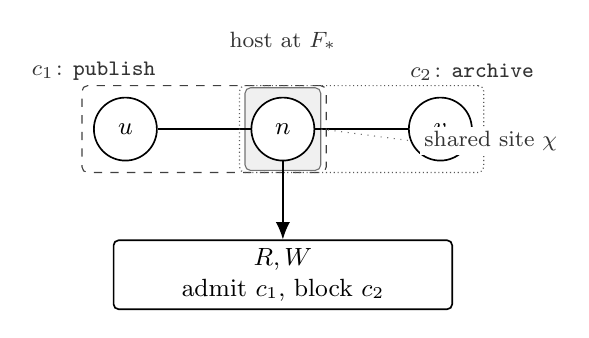
\begin{tikzpicture}[x=1cm,y=1cm]
		\node[host node] (u) at (0,0) {$u$};
		\node[host node] (n) at (2.0,0) {$n$};
		\node[host node] (v) at (4.0,0) {$v$};

		\draw[host edge] (u)--(n)--(v);

		\node[claim A, fit=(u)(n), label={[warp label]above left:$c_1\!:\,\texttt{publish}$}] {};
		\node[claim B, fit=(n)(v), label={[warp label]above right:$c_2\!:\,\texttt{archive}$}] {};
		\begin{scope}[on background layer]
			\node[slice box, fit=(n), minimum width=0.95cm, minimum height=1.05cm] (slice) {};
		\end{scope}

		\node[warp label] at (2,1.12) {host at $F_*$};
		\path (slice.east) ++(1.15,-0.15) coordinate (chiTag);
		\draw[black!55, dotted] (slice.east) -- (chiTag);
		\node[warp label, anchor=west] at ($(chiTag)+(0.10,0)$) {shared site $\chi$};

		\node[warp small, minimum width=4.3cm] (res) at (2,-1.85) {$R, W$\\admit $c_1$, block $c_2$};
		\draw[warp edge] (n.south) -- (res.north);
	\end{tikzpicture}
	\caption{DPO-style overlapping matches over a shared host site \cite{Ehrig2006,Corradini1997}. The two candidates overlap on \(n\), so admission preserves the admitted rewrite together with a witness of the blocked alternative.}
	\label{fig:tick-overlap}
\end{figure}

In this case admission cannot lawfully admit both candidates. A typical result is
that one candidate is admitted, the other is blocked, and the witness \(W\)
records that the candidates overlapped on the same semantic site under an
exclusivity policy. \textbf{Engineering implication.} The receipt is not merely
a log of what happened, but a replayable explanation of why the blocked
candidate could not lawfully coexist in that tick.

Written in optic form, the local scheduler lowers the candidate rewrite bundle
over the shared slice \(\chi\):

\[
	\operatorname{Lower}_{\Psi_{\mathrm{tick}}}(F_*, \{c_1, c_2\})
	=
	(R, W, \theta),
	\qquad
	R \in \{\operatorname{Derived}(c_1), \operatorname{Derived}(c_2)\}.
\]

	The display says exactly that: one candidate becomes the derived result in
	\(R\), while the overlap and blocked coexistence story are preserved in
	\(W\) and retained in \(\theta\), avoiding silent discard.

\subsection{Example 2: A Braid That Remains Plural}

Let two strands \(S_1\) and \(S_2\) share a common parent frontier \(F_*\). Each strand carries a valid claim over the same inherited object, but the claims are incompatible: \(S_1\) records one lawful update to the object, while \(S_2\) records another lawful update that cannot be jointly derived under the braid collapse policy \(\Pi\). The refined braid cells \(\chi\) isolate the shared site together with the local reintegration seams needed for comparison.

Figure~\ref{fig:braid-plural} shows the braid geometry and the preserved plural outcome.

\begin{figure}[H]
	\centering
	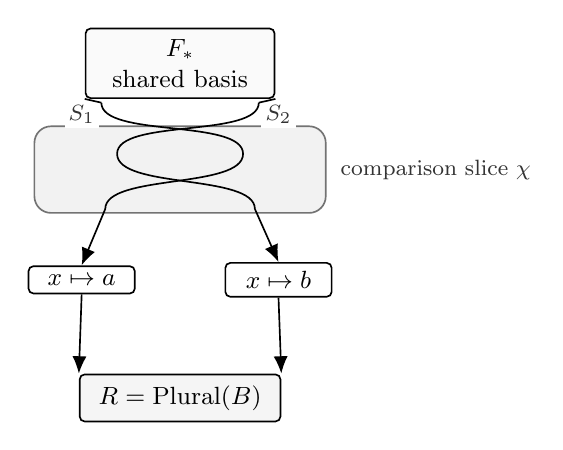
\begin{tikzpicture}[x=1cm,y=1cm]
		\node[warp stage, minimum width=2.4cm] (base) at (2.2,3.3) {$F_*$\\shared basis};
		\node[warp label] at (0.95,2.65) {$S_1$};
		\node[warp label] at (3.45,2.65) {$S_2$};

		\begin{scope}[on background layer]
			\node[warp band, minimum width=3.7cm, minimum height=1.1cm] (band) at (2.2,1.95) {};
		\end{scope}
		\node[warp label, anchor=west] at (4.18,1.95) {comparison slice $\chi$};

		\coordinate (l0) at (1.2,2.8);
		\coordinate (r0) at (3.2,2.8);
		\coordinate (l1) at (3.0,2.15);
		\coordinate (r1) at (1.4,2.15);
		\coordinate (l2) at (1.25,1.45);
		\coordinate (r2) at (3.15,1.45);

		\draw[semithick] (base.south west) -- (l0);
		\draw[semithick] (base.south east) -- (r0);
		\draw[semithick] (l0) .. controls +(0,-0.45) and +(0,0.45) .. (l1)
		.. controls +(0,-0.45) and +(0,0.45) .. (l2);
		\draw[semithick] (r0) .. controls +(0,-0.45) and +(0,0.45) .. (r1)
		.. controls +(0,-0.45) and +(0,0.45) .. (r2);

		\node[warp small, minimum width=1.35cm] (a) at (0.95,0.55) {$x\mapsto a$};
		\node[warp small, minimum width=1.35cm] (b) at (3.45,0.55) {$x\mapsto b$};
		\node[warp shell, minimum width=2.55cm] (plural) at (2.2,-0.95) {$R=\mathrm{Plural}(B)$};

		\draw[warp edge] (l2) -- (a.north);
		\draw[warp edge] (r2) -- (b.north);
		\draw[warp edge] (a.south) -- (plural.north west);
		\draw[warp edge] (b.south) -- (plural.north east);
	\end{tikzpicture}
	\caption{Two strands literally braid over a shared basis. The resulting claims remain plural when no lawful collapse exists under the braid policy.}
	\label{fig:braid-plural}
\end{figure}

The important point is that the lawful outcome may remain \texttt{Plural}. When
collapse lacks lawful justification to choose between the two claims, plurality
itself is the correct admitted result under the governing policy. The witness
then preserves both the fact of divergence and the fact that preserved plurality
was the lawful outcome. \textbf{Engineering implication.} Branch structure can
remain representationally honest: disagreement can persist as plurality instead
of being forced into a premature merge.

Written in optic form, collapse over the braid looks like this:

\[
	\operatorname{Lower}_{\Psi_{\mathrm{braid}}}(F_*, B)
	=
	(R, W, \theta),
	\qquad
	R = \operatorname{Plural}(B).
\]

The display shows that \(R\) may remain plural. Plurality is itself a lawful
lowered result, with the witness and retained hologram explaining why further
collapse lacked justification over that bounded comparison slice.

\subsection{Example 3: Transport Before Import}

Let replicas \(R_A\) and \(R_B\) share a common prefix \(F_*\). Replica \(R_A\)
has admitted a suffix \(\sigma_A\) beyond that prefix, and replica \(R_B\) wishes
to import it. Let \(F_B\) denote \(R_B\)'s present comparable frontier. The
relevant weave is the family of transported remote claims derived from
\(\sigma_A\). The bounded site \(\chi\) is the imported region together with the
local context needed to decide whether the import remains lawful at \(R_B\)'s
present basis.

Figure~\ref{fig:transport-before-import} makes the transport-before-import order explicit.

\begin{figure}[H]
	\centering
	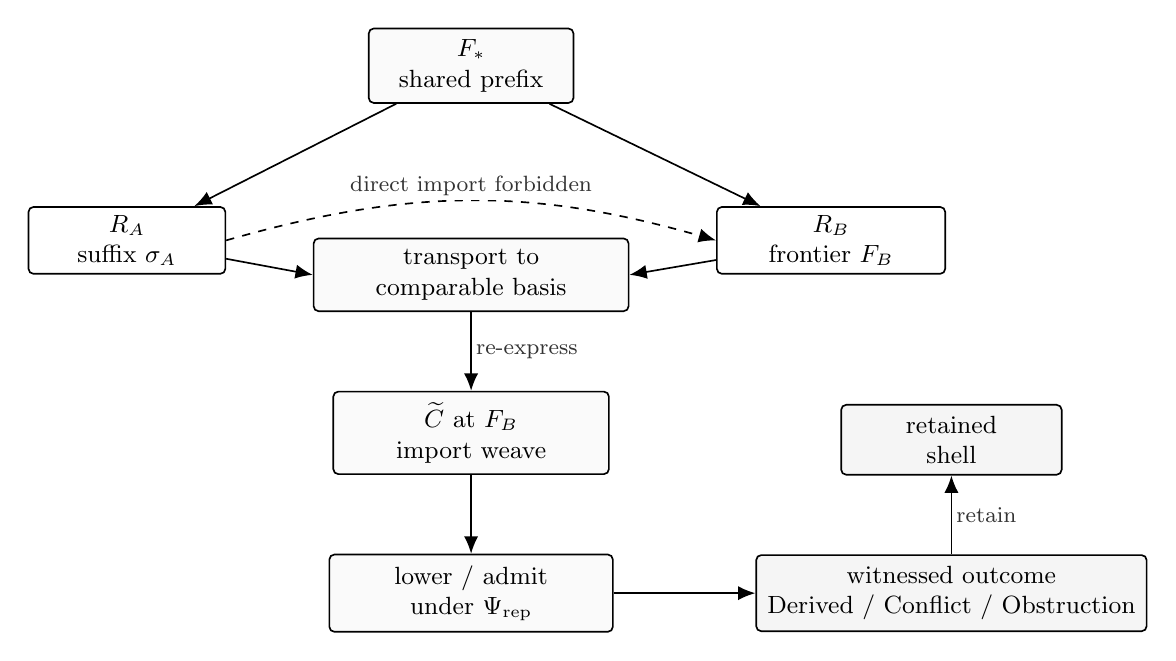
\begin{tikzpicture}[node distance=10mm and 14mm]
		\node[warp stage, minimum width=2.6cm] (shared) {$F_*$\\shared prefix};
		\node[warp small, minimum width=2.5cm, below left=13mm and 18mm of shared] (src) {$R_A$\\suffix $\sigma_A$};
		\node[warp small, minimum width=2.9cm, below right=13mm and 18mm of shared] (recv) {$R_B$\\frontier $F_B$};

		\node[warp stage, minimum width=4.0cm, below=17mm of shared] (transport) {transport to\\comparable basis};
		\node[warp stage, minimum width=3.5cm, below=10mm of transport] (weave) {$\widetilde C$ at $F_B$\\import weave};
		\node[warp stage, minimum width=3.6cm, below=10mm of weave] (lower) {lower / admit\\under $\Psi_{\mathrm{rep}}$};
		\node[warp shell, minimum width=4.5cm, right=18mm of lower] (out) {witnessed outcome\\Derived / Conflict / Obstruction};
		\node[warp shell, minimum width=2.8cm, above=10mm of out] (shell) {retained\\shell};

		\draw[warp edge] (shared) -- (src);
		\draw[warp edge] (shared) -- (recv);
		\draw[warp edge] (src) -- (transport.west);
		\draw[warp edge] (recv) -- (transport.east);
		\draw[warp dashed] (src.east) to[bend left=16] node[warp label, above] {direct import forbidden} (recv.west);
		\draw[warp edge] (transport) -- node[warp label, right] {re-express} (weave);
		\draw[warp edge] (weave) -- (lower);
		\draw[warp edge] (lower) -- (out.west);
		\draw[warp edge] (out.north) -- node[warp label, right] {retain} (shell.south);
	\end{tikzpicture}
	\caption{A remote suffix cannot be judged directly at the receiver's tip; it must first be transported to a comparable basis.}
	\label{fig:transport-before-import}
\end{figure}

Transport first re-expresses the remote suffix at a comparable frontier. Once
that transported weave exists, the replica optic can lawfully lower it. If
transport or lowering fails, the result is conflict or obstruction with an
explicit witness. \textbf{Engineering implication.} Replication becomes
queryable and auditable as lawful transport and lowering.

Written in optic form, the order of acts matters:

\[
	\begin{aligned}
		\widetilde{C}
		 & =
		\operatorname{Transport}(F_*, \sigma_A, F_B),                   \\
		(R, W, \theta)
		 & =
		\operatorname{Lower}_{\Psi_{\mathrm{rep}}}(F_B, \widetilde{C}), \\
		R
		 & \in
		\{\operatorname{Derived}(x), \operatorname{Conflict}, \operatorname{Obstruction}\}.
	\end{aligned}
\]

The first line localises the hard part in transport: the remote suffix is
re-expressed at a comparable frontier before any import judgement is attempted.
The second line then lowers the replica-scale weave under
the same optic shape already trusted locally. The third line makes explicit
that even after successful normalisation, the lowered outcome may still be
derivation, conflict, or obstruction.

\clearpage
\section{Continuum and the Post-Unix Horizon}

We use \emph{Continuum} to name the protocol-shaped causal medium induced by
witnessed admission. Continuum is not a privileged runtime standing above any
participant. It is the shared medium formed by exchangeable witness-bearing
artefacts---suffixes, shells, receipts, and certificates---together with the
transport rules that re-express remote history at comparable bases so that the
downstream optic can be lowered lawfully.

Because tick admission, braid collapse, and replica import share one optic law,
it becomes natural to treat operating-system objects as frontier-relative
materialisations over that same causal medium.

The post-Unix claim of the paper is not that the operating system becomes graph-shaped. It is that the operating system becomes frontier-relative.

The relevant lineage is Unix's process/file discipline, capability systems' authority discipline, and Plan 9's namespace discipline; \WARP{} shifts the centre of gravity from container, descriptor, or address space to witnessed causal admission over shared history \cite{RitchieThompson1974,DennisVanHorn1966,Levy1984,Pike1995}.

A tempting but inadequate shorthand would be to say that a process
\emph{is} a divergent worldline. That collapses history, live realisation, and
working-set materialisation into one object. The sharper formulation is that a
process is a strand whose live realisation appears as a shadow working set over
shared machine history. The process is the active frontier-relative
manifestation of one strand over that history.

This changes the meaning of ownership, isolation, deletion, debugging, and restart. Safety is no longer a byproduct of process opacity. It becomes a property of lawful admission over semantically closed sites. If shared history is primary, the privacy problem becomes explicit as well: the system must provide a protected interval in which exploratory work does not immediately become collaborative fact.

\subsection{Application Boundary}
The same post-Unix shift also changes how applications should meet the runtime.
The relevant question is no longer how to add handwritten app methods to a host.
It is how to compile app-authored optic surfaces into lawful set-side intents
and lawful get-side observer plans over one generic holographic runtime. In
that arrangement, the application authors its own nouns, result families, and
reading families; a compiler lowers those surfaces into intent envelopes,
observer plans, and shared codecs; and the runtime remains generic, admitting
	intents, emitting outcome/receipt/hologram boundaries, and later serving
	bounded readings through hosted observers. We do not formalise that
	compiler boundary here. The architecture developed here places it at a clear
	engineering seam.

	Figure~\ref{fig:sdl-compiler-runtime} sketches that seam.

\begin{figure}[H]
	\centering
	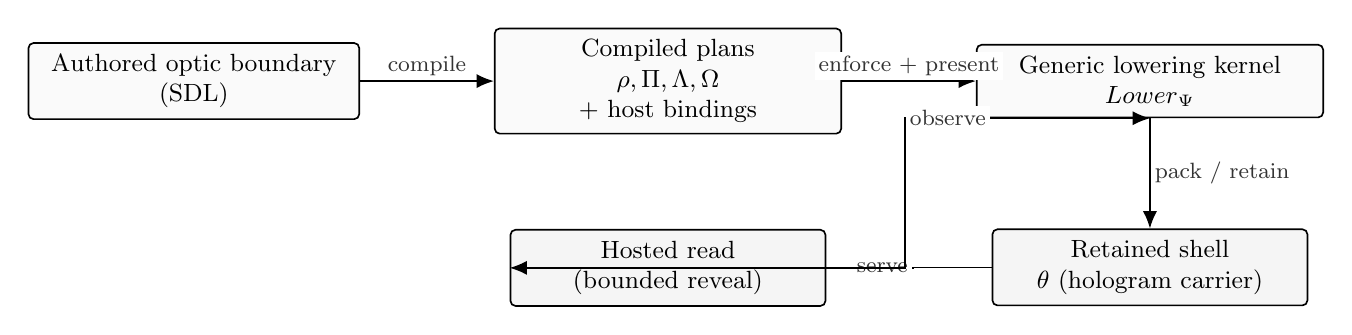
\begin{tikzpicture}[x=1cm,y=1cm, every node/.style={font=\small}]
		% ER-style: show stable objects and relations at the seam.
		\node[warp stage, minimum width=4.2cm] (sdl) at (0,0)
		{Authored optic boundary\\(SDL)};

		\node[warp stage, minimum width=4.4cm, right=17mm of sdl] (plans)
		{Compiled plans\\\(\rho,\Pi,\Lambda,\Omega\)\\+ host bindings};

		\node[warp stage, minimum width=4.4cm, right=17mm of plans] (kernel)
		{Generic lowering kernel\\\(\operatorname{Lower}_\Psi\)};

		\node[warp shell, minimum width=4.0cm, below=14mm of kernel] (shell)
		{Retained shell\\\(\theta\) (hologram carrier)};

		\node[warp shell, minimum width=4.0cm, below=12mm of plans] (read)
		{Hosted read\\(bounded reveal)};

		\draw[warp edge] (sdl) -- node[warp label, above] {compile} (plans);
		\draw[warp edge] (plans) -- node[warp label, above] {enforce + present} (kernel);
		\draw[warp edge] (kernel) -- node[warp label, right] {pack / retain} (shell);
		\draw[warp edge] (shell.west) -- ++(-1.0,0) |- node[warp label, left] {serve} (read.west);
		\draw[warp edge] (read.east) -- ++(1.0,0) |- node[warp label, right] {observe} (kernel.south);
	\end{tikzpicture}
	\caption{Authored optic boundaries compile into generic admission and observer machinery.}
	\label{fig:sdl-compiler-runtime}
\end{figure}

\subsection{Example: An Authored Hot-Text Optic}
We make that application boundary concrete by looking at a small
developer-authored hot-text boundary. The
full SDL declares the hot nouns of one text layer---\texttt{BufferWorldline},
\texttt{RopeHead}, \texttt{RopeBranch}, \texttt{RopeLeaf}, \texttt{TextBlob},
\texttt{Anchor}, \texttt{Tick}, \texttt{TickReceipt}, and
\texttt{Checkpoint}---together with a small family of read and write surfaces
over them. The paper prints one representative rewrite and omits the full
schema. Although this boundary is written in GraphQL SDL, it is not a claim
that a canonical graph object sits underneath the editor. It is a convenient
authoring syntax for an optic boundary: a typed aperture over one hot layer and
its admissible rewrite surfaces.

GraphQL was selected here for deliberate reasons. It lets application authors
declare the hot nouns of a layer and the admissible rewrite surfaces over them
in one typed schema. That in turn allows a schema compiler---in the current
toolchain---to check footprint obligations, slot bindings, and forbidden
reachability at compile time, before arbitrary host code has run.
Just as importantly, the SDL narrows the authoring surface:
the developer is declaring shapes, closures, and mutations, not smuggling in
ambient non-determinism through random sources, wall-clock reads, or hidden
side effects. GraphQL is also easy to version, so new nouns, rewrites, and
migrations can be staged as explicit schema evolution, avoiding silent runtime
drift.
We treat GraphQL here as an authoring surface; its use as an API and query
language is standard \cite{GraphQLSpec}.

The central rewrite in that family is \texttt{replaceRangeAsTick}, because it
shows the optic shape with minimal extra machinery:

\paragraph{From surface to runtime admission.}
Compilation of a surface like \texttt{replaceRangeAsTick} yields a typed intent
envelope (carrying arguments plus declared reads/writes/creates/forbids) and
generated host bindings that enforce those declarations. At runtime, the generic
lowering kernel uses the declared closures to construct the bounded slice
\(\chi\), applies the admissibility law \(\Pi\) over the presented claim family,
and packs the declared receipt and retention obligations under \(\Lambda\).

\begin{lstlisting}[style=aioncode]
replaceRangeAsTick(
  input: ReplaceRangeAsTickInput!
): ReplaceRangeAsTickResult!
    @wes_op(name: "replaceRangeAsTick")
    @wes_footprint(
    reads: [
      "BufferWorldline"
      "RopeHead"
      "RopeBranch"
      "RopeLeaf"
      "TextBlob"
      "Anchor"
    ]
    writes: ["BufferWorldline"]
    creates: [
      "TextBlob"
      "RopeLeaf"
      "RopeBranch"
      "RopeHead"
      "Tick"
      "TickReceipt"
    ]
    slots: [
      {
        slot: "worldline"
        kind: "BufferWorldline"
        bindFromArg: "input.worldlineId"
        access: [READ, WRITE]
      }
      {
        slot: "baseHead"
        kind: "RopeHead"
        bindFromArg: "input.baseHeadId"
        access: [READ]
      }
    ]
    closures: [
      {
        slot: "touchedRope"
        fromSlot: "baseHead"
        operator: "ropeRangeClosure"
        argBindings: ["input.startByte", "input.endByte"]
        reads: ["RopeBranch", "RopeLeaf", "TextBlob"]
        cardinality: MANY
      }
      {
        slot: "affectedAnchors"
        fromSlot: "worldline"
        operator: "anchorsIntersectingEditWindow"
        argBindings: ["baseHead", "input.startByte", "input.endByte"]
        reads: ["Anchor"]
        cardinality: MANY
      }
    ]
    createSlots: [
      { slot: "newBlob", kind: "TextBlob", cardinality: OPTIONAL }
      { slot: "newLeaves", kind: "RopeLeaf", cardinality: MANY }
      { slot: "newBranches", kind: "RopeBranch", cardinality: MANY }
      { slot: "nextHead", kind: "RopeHead" }
      { slot: "tick", kind: "Tick" }
      { slot: "receipt", kind: "TickReceipt" }
    ]
    updates: [{ slot: "worldline", fields: ["canonicalHead"] }]
    forbids: ["AstState", "Diagnostics", "GitWitness", "UiState"]
    )
\end{lstlisting}

	This is exactly the developer-facing form of a \WARP{} optic. The authored
	surface names the hot nouns that matter, the closure operators that construct
	the optic slice, the created causal consequences that the runtime must retain,
	and the materialised reading that may change. The operation
	\texttt{replaceRangeAsTick} defines a bounded rewrite surface over a buffer
	worldline.
	The closures \texttt{ropeRangeClosure} and
	\texttt{anchorsIntersectingEditWindow} construct the local slice to be judged;
	the created \texttt{Tick} and \texttt{TickReceipt} make the witness-bearing
	consequences explicit; and the \texttt{forbids} clause makes the aperture
	explicit by ruling out silent dependence on AST state, diagnostics, Git witness
	history, or UI state.

We omit the full SDL. Our goal here is to show the authored pattern.
	Even this one excerpt is enough to expose it: the developer declares
	the nouns in scope, the closures that build the local slice, the causal
	consequences that must be retained, the materialised reading that may change,
	and the regions that remain outside the aperture. In ordinary software a
	developer might declare methods over mutable structures. In a \WARP{}-native
	system, the more faithful statement is that the developer authors optic
	boundaries and lets a schema compiler compile those boundaries
	into runtime-checkable footprint, witness, and retention obligations.

\subsection{The Three-Tier Thinking Room}

Continuum remains socially viable only if retention and revelation are decoupled. Shared history creates exposure pressure that a simple public/private split cannot absorb: users need room to think, to speculate, and only later to promote. We therefore distinguish a protected working interval with three practical tiers:

\begin{enumerate}[leftmargin=*]
	\item \textbf{Ephemeral Scratch}: local, weakly retained, and disposable.
	\item \textbf{Author-Only Speculative Lane}: durable, replayable, sealed to the author by default.
	\item \textbf{Shared / Admitted Lane}: collaboratively admitted causal truth.
\end{enumerate}

This is the privacy-preserving answer to the exposure pressure created by shared
causal history. The system may remember drafts, with revelation and retention
governed by explicit policy and tier. Architecturally, Ephemeral Scratch is
pre-admission or minimally retained local work; Author-Only lanes are durable
and replayable prior to social transport; Shared lanes mark the moment private
speculation crosses into collaborative truth.

This distinction matters immediately for debugger-driven counterfactual work. A
reading, replay, or inspection act is revelation only. It does not by itself
create new causal truth. If an operator explicitly asks to continue from an
earlier coordinate or explore a counterfactual alternative, the system should
emit an explicit fork rooted at an exact fork basis. Such debugger-created
strands are real causal objects; they should default to Ephemeral Scratch or an
Author-Only Speculative Lane until an explicit promotion moves them into shared
history. When retained, their provenance should record the creating principal,
tool or session origin, fork basis, and retention or revelation posture.

\clearpage
\section{Privacy, Provenance, and Revelation}

Privacy and provenance are not mutually exclusive \cite{Ross2026VI}. We do not
re-derive that machinery here. The present point
is to show how its privacy, revelation, and observer-rights discipline inhabits
the generic hologram and retained-contract structure of the \WARP{} optic.
Three components matter.

\subsection{Property Library}

Private speculative lanes can collaborate without exposing their full internal
history. This is where proof-bearing evidence, proof-carrying certification,
information-flow control, and zero-knowledge style selective disclosure touch
the architecture \cite{MartinLof1984,Necula1997,Denning1976,Goldwasser1989}.
They emit a certificate of lawfulness: property-bearing evidence that
type/resource safety, admission integrity, provenance linkage, and policy
conformance hold at the required tier. Such a certificate should minimally
identify the shared basis to which it refers, the property set it attests, the
witness or proof tier under which those properties were established, and the
shell anchors needed for later replay, audit, or revocation. In that sense the
certificate is a special case of the generic package \(\theta\): a carrier of
witness-bearing consequences upon which others may lawfully rely. Some
properties may survive fold-to-opaque as shell anchors or zero-knowledge proofs;
others, such as full forensic traces, require later unsealing.

One compact lifecycle makes the point concrete. A private lane may first
\emph{issue} a certificate stating, for example, that a bounded build or data
preparation step satisfies a declared policy at basis \(F_*\). The certificate
then becomes \emph{active} once the relevant principal, witness tier, and
retention contract are all in force. A collaborator may subsequently
\emph{rely} on that certificate without receiving the sealed internal trace
itself, because the relied-upon shell anchors and property set are already
named. If later evidence shows that the attested condition no longer holds, the
certificate may be \emph{revoked} by a new witnessed status transition that
changes future lawful reliance without deleting past history. Finally, the
certificate may be \emph{archived}, preserving its basis, attested properties,
and revocation history for later audit even when it is no longer active for
ordinary use.

\subsection{Reliance Status}

Once certificates exist, trust itself becomes a first-class object with a
lifecycle, echoing the pressure visible in PKI and certificate revocation
systems while generalising the object being trusted \cite{RFC5280}. A
certificate can be issued, activated, superseded, suspended, revoked, expired,
and archived. Revocation is not deletion. It is a new witnessed status
transition about future lawful reliance. This creates a true reliance domain
within \WARP{} and makes trust an internal witnessed object.

One concrete case is a collaborator relying on an active certificate that
attests a sealed build, data preparation step, or model export at basis
\(F_*\). While the certificate remains active, downstream admissions may rely
on that shell and its property set without reopening the sealed internal trace.
If the certificate is later suspended or revoked because an upstream witness is
invalidated, future lawful reliance must stop immediately even though the
earlier basis, reliance events, and revocation act remain replayable and
auditable.

\subsection{Observer Rights}

The subject-side counterpart is an observer rights lattice governing who may
discover, inspect, rely on, unseal, replay, export, delegate, or revoke access
over proof-bearing artefacts. The right local noun here is not ``lens'' but
``reading'': an observer, equipped with a bounded reading frame, obtains a
lawful projection by decoding only the least required slice of a subject's
backward causal cone. In this ontology, that reading is a coordinate chart
over causal history. Different observers may therefore lawfully emit different
charts over the same history, and revelation law must govern which transitions
between such charts are permitted, what witness must travel with them, and what
plurality or obstruction must remain explicit. This is where the architecture
meets the observer classes, replay impact labels, and bounded warrants developed
elsewhere in the series.
High-impact revelation rights should be activated explicitly, often requiring
threshold or role-separated co-authorisation.

A simple rights split makes the point concrete. The author of a private lane may
hold replay and unseal rights over the full trace. A teammate may hold only the
right to inspect the active certificate and summary shell. A release principal
may be permitted to request wider revelation, but only under co-authorised
unsealing. The architecture therefore does not ask one observer class to serve
every use. It lets lawful readings differ by right, scope, and witness tier.

\clearpage
\section{Open Frontier Questions}

The architectural centre is stable enough that the remaining work can be stated
as extension rather than as hidden prerequisite. The next frontier laws likely
fall into two clusters.

\paragraph{Governance and reliance laws.}
\begin{itemize}[leftmargin=*]
	\item \textbf{exposure ledger and contamination calculus},
	\item collective sovereignty over co-owned traces,
	\item mode-transition contamination and stale certificate handling,
	\item \textbf{revocation propagation over dependency graphs},
	\item aperture decay as a witnessed act,
	\item temporal-logic query languages over lawful transport, admission, and revelation paths.
\end{itemize}

\paragraph{Engineering seams.}
\begin{itemize}[leftmargin=*]
	\item lawful compilation of app-authored optics into intent and observer plans,
	\item settlement shells and idempotent import of already-adjudicated outcomes,
	\item export semantics at the causal-medium boundary.
\end{itemize}

These points become visible once the foundations are coherent enough to support
a real social-runtime theory. The final paper should therefore turn from the
internal recurrence of the \WARP{} optic to the external consequence of that
recurrence: there is no primary runtime. If graph-like state is an
observer-relative reading and replica import is ordinary witnessed admission,
then Continuum is not a runtime standing above any participant. It is the
protocol-shaped causal medium defined by witnessed suffixes, transport, slicing,
lowering, outcome algebra, and bounded revelation.
Paper VIII develops that consequence directly: Continuum is a protocol of
witnessed admission, not a privileged runtime.

\clearpage
\section{Conclusion}

The central result of this paper is a clearer object. \WARP{} is an optic
architecture in which state transitions, braid outcomes, certificate trust,
historical folding, and observer revelation are treated as instances of the same
witnessed act: project through an observer, bound an optic slice, lawfully lower
a weave, and retain the result as a hologram. Because each recurrence emits such
a hologram, replay, audit, transport, and counterfactual examination recur as
well. Every retained slice contains the least sufficient history of its bounded
admitted situation up to the governing retention contract. Tick replay is
therefore only the first concrete instance of a more general property that also
appears in braid lowering, distributed import, and later trust-bearing shells.

The distributed consequence is correspondingly precise. Transport constructs the
comparable slice on which replica-scale lowering can occur; once that slice
exists, the downstream optic is the same one already used locally.
Distribution changes the slice boundary while leaving the downstream law
unchanged.

That optic still requires judgement and interpretation. It does, however, make
the terms of collaboration explicit: what plural situation was lowered, over
what site, under what policy, with what retained witness, and under what
revelation rights. In a \WARP{}-native system, when software executes, it
commits, folds, and reveals truth under law.

\clearpage
\appendix

\section{Adversarial Transport (Sketch)}

The main text treats replica transport as a normalisation step that constructs a
comparable basis and re-expresses a remote suffix family as a weave suitable for
lowering. This appendix records the minimal obligations we expect transport to
satisfy under hostile distributed conditions. The goal is not a complete
protocol or a full formalisation; it is to keep the architectural interface
honest about what ``transport'' must supply so that the replica optic can either
lower lawfully or return an explicit \texttt{Conflict} or \texttt{Obstruction}.

\subsection{Threat model}

We assume:
\begin{itemize}[leftmargin=*]
	\item an untrusted network that may reorder, delay, duplicate, or drop
	      messages;
	\item remote replicas that may be faulty, partially connected, or actively
	      adversarial (including equivocation) \cite{LamportShostakPease1982};
	\item bounded local resources, so a receiver must remain able to refuse work
	      that exceeds its admitted slice and retention posture.
\end{itemize}
We do not assume a global reliable broadcast or a synchronous network
\cite{Bracha1987}. We also do not assume that all participants share the same
authority regime; trust and reliance are part of the witness-bearing objects,
not ambient background.

\subsection{Transport obligations}

At replica scale, the lowering surface \(\rho_{\mathrm{replica}}\) uses
\(\operatorname{Transport}\) to construct a weave \(\widetilde{C}\) at a
receiving comparable frontier. Under hostile conditions, that construction must
provide at least:
\begin{itemize}[leftmargin=*]
	\item \textbf{Authorship evidence}: a proof-carrying identity for the claimed
	      remote suffix family and its basis anchors (for example signatures or
	      certificate chains), sufficient for the receiver's authority regime to
	      decide whether reliance is permitted at all.
	\item \textbf{Basis comparability}: an explicit description of the basis
	      anchors and transport path used to re-express the remote claims at the
	      receiver's comparable frontier. If comparability cannot be established,
	      transport yields \texttt{Obstruction}.
	\item \textbf{Witness carriage}: a witness tier sufficient for replay, audit,
	      and later revocation or dispute. Transport must not erase the ability to
	      explain why a later import was admitted, blocked, or obstructed.
	\item \textbf{Idempotence keys}: stable identifiers for transported claim
	      families and their derived settlement shells, so that duplicate delivery
	      can be treated as replay of an already witnessed object.
\end{itemize}

These obligations do not solve adversarial transport. They make its inputs and
outputs explicit enough that downstream lowering remains lawful and auditable.

\subsection{Failure modes and lawful outcomes}

Hostile and failure-path behaviour should surface as witnessed outcomes instead
of being absorbed as silent heuristics:
\begin{itemize}[leftmargin=*]
	\item \textbf{Unauthenticated claims}: transport returns \texttt{Obstruction}
	      with a witness explaining the missing or insufficient evidence.
	\item \textbf{Equivocation}: when a principal authors incompatible remote
	      suffix families over the same basis, the receiver treats the situation
	      as a lawful \texttt{Conflict} or a policy-driven \texttt{Obstruction},
	      and emits a witness suitable for later revocation or quarantine.
	\item \textbf{Partial connectivity}: missing dependencies, missing basis
	      anchors, or incomplete transported slices return \texttt{Obstruction}
	      rather than speculative patch application.
	\item \textbf{Replay and duplication}: duplicate delivery becomes idempotent
	      re-introduction of the same witnessed transport object, not a new
	      authored intent.
	\item \textbf{Resource exhaustion}: when a transported family would force a
	      receiver beyond its bounded slice \(\chi\), retention contract
	      \(\Lambda\), or authority regime \(\alpha\), the receiver may lawfully
	      obstruct the import at the boundary.
\end{itemize}

\subsection{Architectural consequence}

The replica-scale doctrine remains the same: transport constructs the comparable
slice and produces a weave; lowering judges that weave under the governing optic
and retention contract. Under hostile conditions, transport and authority decide
whether the imported object is admissible for judgement at all. The outcome is
therefore witnessed: \texttt{Derived} when import succeeds, \texttt{Conflict}
when incompatibility is surfaced, and \texttt{Obstruction} when preconditions
fail.

\clearpage
\section{WARP Glossary}

This glossary gathers the recurring nouns of this paper and the surrounding
series. The entries are intentionally architectural and implementation-agnostic.

\begingroup
\footnotesize
\setlength{\tabcolsep}{3.5pt}
\renewcommand{\arraystretch}{0.97}

\subsection{Symbolic Vocabulary}

\begin{center}
	\begin{tabularx}{\textwidth}{@{}>{\raggedright\arraybackslash}p{0.26\textwidth}X@{}}
		\toprule
		Symbol                                                                                                                                          & Meaning                                                                                                                                                      \\
		\midrule
		\(\Omega = (\pi,\beta,M,U,E)\)                                                                                                                  & Observer plan: projection, basis, observer state, update discipline, and emission.                                                                           \\
		\(\Psi = (\Omega,\chi,\rho,\Pi,\Lambda)\)                                                                                                       & \WARP{} optic: observer plan, optic slice, set-side lowering surface, admissibility law, and retention contract.                                             \\
		\(\mathcal{P}\)                                                                                                                                 & Basis-relative weave. Depending on scale, this may be a candidate rewrite bundle, a braid, or a transported import family.                                   \\
		\(\rho(F_*, \mathcal{P}; \Omega) = (C,\chi)\)                                                                                                   & Set-side lowering surface presenting comparable claims \(C\) over bounded slice \(\chi\) from weave \(\mathcal{P}\) at frontier \(F_*\).                     \\
		\(\operatorname{Lower}_{\Psi}(F_*, \mathcal{P}) = (R,W,\theta)\)                                                                                & Full optic act: lower weave \(\mathcal{P}\) under optic \(\Psi\) at frontier \(F_*\), yielding outcome \(R\), witness \(W\), and hologram \(\theta\).        \\
		\(\mathcal{O}(X) = \operatorname{Derived}(X) \sqcup \operatorname{Plural}(X) \sqcup \operatorname{Conflict} \sqcup \operatorname{Obstruction}\) & Outcome algebra for lawful lowering over scale-local carrier \(X\).                                                                                          \\
		\(\theta \simeq_{\Lambda} \theta'\)                                                                                                             & Shell equivalence under retention contract \(\Lambda\). Equivalent shells preserve the same optic-accurate bulk for the lawful uses demanded by \(\Lambda\). \\
		\(\operatorname{Transport}(F,\Sigma,F')\)                                                                                                       & Replica-scale basis construction: re-express remote suffix family \(\Sigma\) from frontier \(F\) at comparable frontier \(F'\) before lowering.              \\
		\(\operatorname{Commit}_{\Psi}(F_*, \mathcal{P})\)                                                                                              & Commitment act: shorthand for optic lowering when the lowered result is being treated as admitted frontier-relative truth.                                   \\
		\(\operatorname{Fold}_{\Lambda}(\theta)\)                                                                                                       & Fold a shell into a \(\Lambda\)-equivalent retained carrier.                                                                                                 \\
		\(\operatorname{Reveal}_{\Omega,\alpha}(m,\theta)\)                                                                                             & Revelation act under observer plan \(\Omega\), authority regime \(\alpha\), observer state \(m\), and shell \(\theta\).                                      \\
		\bottomrule
	\end{tabularx}
\end{center}

\subsection{History And Lane Nouns}

\begin{center}
		\begin{tabularx}{\textwidth}{@{}>{\raggedright\arraybackslash}p{0.26\textwidth}X@{}}
			\toprule
			Term           & Meaning                                                                                                                                                                                                                     \\
			\midrule
	\WARP{}        & An optic architecture over shared causal history. The system's primary object is witnessed causal history, with frontier-relative materialisations over it.                                                                        \\
			Continuum      & The protocol-shaped causal medium formed by exchangeable witness-bearing artefacts (suffixes, shells, receipts, certificates) and the transport rules that make remote history comparable for lawful lowering.                        \\
			Causal lane    & A history-bearing computational object. The ontology-level noun for a causal line of development, whether canonical or speculative.                                                                                         \\
			Worldline      & A canonically admitted causal lane. Its history and frontier-relative materialisations count as shared causal reality for the relevant policy frame.                                                                        \\
			Strand         & A speculative causal lane rooted at a parent worldline and fork anchor, carrying lawful local divergence over inherited history.                                                                                            \\
	Braid          & A lane-scale weave over multiple lanes sharing a common precursor or basis, presented for comparison and later collapse under policy.                                                                                          \\
		Weave          & A basis-relative carrier that holds multiple candidate claims in suspension without yet forcing one derived answer. Candidate rewrite bundles, braids, and transported import families are the primary cases in this paper. \\
		Frontier       & The coordinate at which a lane or materialisation is interpreted. A frontier-relative view changes with the chosen basis.                                                                                                   \\
		Basis          & The comparison or reading coordinate relative to which claims, slices, or observers are made commensurable.                                                                                                                 \\
		Fork anchor    & The exact inherited basis at which a strand diverges from a parent worldline.                                                                                                                                               \\
		Shared history & The admitted causal medium from which frontier-relative readings are materialised.                                                                                                                                          \\
		\bottomrule
	\end{tabularx}
\end{center}

\subsection{Admission And Replay Nouns}

\begin{center}
	\begin{tabularx}{\textwidth}{@{}>{\raggedright\arraybackslash}p{0.26\textwidth}X@{}}
		\toprule
		Term                       & Meaning                                                                                                                                                                                    \\
		\midrule
		Claim family \(C\)         & The comparable claim presentation produced by an optic's set-side lowering surface over a bounded slice.                                                                                   \\
		Policy \(\Pi\)             & The governing law under which a bounded site is judged.                                                                                                                                    \\
		Optic slice \(\chi\)       & The least frontier-relative closure over which the optic can lawfully compare the claims and judge their coexistence, derivation, plurality, conflict, or obstruction.                     \\
		Lowering                   & The set-side act by which an optic lawfully judges a weave over a bounded slice and emits outcome, witness, and hologram.                                                                  \\
		Derived                    & An outcome in which a lawful result is admitted as the derived local or imported result.                                                                                                   \\
Plural                     & An outcome in which plurality itself is the lawful admitted result.                                                                                                                         \\
Conflict                   & An outcome in which the system surfaces genuine incompatibility as an explicit result.                                                                                                     \\
Obstruction                & An outcome in which lawful admission cannot proceed because the relevant preconditions or transport conditions are not satisfied.                                                          \\
Witness \(W\)              & The semantic explanation of why a lowering outcome was lawful. It behaves as proof-bearing residue that supports replay, audit, and explanation.                                            \\
		Shell \(\theta\)           & The retained carrier packaging a lowered result together with witness-bearing consequences for replay, audit, transport, or revelation.                                                    \\
		WARP hologram              & A retained shell preserving the least sufficient boundary needed to recover the optic-accurate bulk of a bounded admitted situation for the required contract.                             \\
		Boundary Transition Record & One concrete shell family, especially at tick scale, used to retain replayable local transition boundaries.                                                                                \\
		Transport                  & The replica-scale normalisation step that re-expresses a remote suffix at a comparable frontier before import judgement.                                                                   \\
		Normaliser                 & The basis-construction step inside an optic's set-side lowering surface. At replica scale, the hard case is transport.                                                                     \\
		Optic-accurate bulk        & The retained causal content, together with the required witness structure, that must remain recoverable for the observations and obligations named by an optic and its retention contract. \\
		\bottomrule
	\end{tabularx}
\end{center}

\subsection{Commitment, Revelation, And Governance Nouns}

\begin{center}
	\begin{tabularx}{\textwidth}{@{}>{\raggedright\arraybackslash}p{0.26\textwidth}X@{}}
		\toprule
		Term                                   & Meaning                                                                                                                                                                                                        \\
		\midrule
		Optic                                  & The composite act by which an observer bounds a site through an aperture, a weave is lawfully lowered there, and the resulting admitted situation is retained as a holographic witness in append-only history. \\
		Commitment                             & The act by which the witnessed outcome of lawful lowering is admitted into frontier-relative truth, whether derivation, plurality, conflict, or obstruction.                                                   \\
		Folding                                & Re-expression of already admitted history into a boundary-equivalent retained shell under an explicit contract.                                                                                                \\
			Revelation                             & Lawful exposure of admitted or folded history to a bounded observer under an aperture and authority regime.                                                                                                    \\
			Observer plan \(\Omega\)               & The revelation-side object specifying projection, basis, accumulation state, update discipline, and emission.                                                                                                  \\
			Observer                               & A positioned reading discipline that determines which readings may be lawfully emitted at a given aperture, basis, and authority tier.                                                                         \\
			Reading                                & A lawful emitted chart over causal history obtained through a bounded observer frame.                                                                                                                          \\
			Aperture                               & The bounded observational scope within which a reading is lawful.                                                                                                                                              \\
			Retention contract \(\Lambda\)         & The obligations a retained shell must continue to satisfy for replay, audit, transport, revelation, or reliance review.                                                                                        \\
			Authority regime \(\alpha\)            & The active rights and reliance discipline governing revelation.                                                                                                                                                \\
			Shell equivalence \(\simeq_{\Lambda}\) & Equivalence between shells relative to the retained contract \(\Lambda\), defined by preservation of lawful replay, audit, transport, or revelation obligations, independent of byte identity.                \\
		Property certificate                   & A proof-bearing shell attesting that specified properties hold relative to a shared basis and witness tier.                                                                                                    \\
		Reliance status                        & The lifecycle state of a certificate or trust-bearing object: issued, active, superseded, suspended, revoked, expired, or archived.                                                                            \\
		Observer rights                        & The rights lattice governing who may inspect, replay, export, delegate, unseal, or revoke access over retained artefacts.                                                                                      \\
		Ephemeral Scratch                      & Local, weakly retained, disposable work that has not yet crossed into durable collaborative history.                                                                                                           \\
		Author-Only Speculative Lane           & Durable, replayable, but author-sealed speculative work that has not yet been socially transported.                                                                                                            \\
		Shared / Admitted Lane                 & The portion of history that has crossed into collaboratively admitted causal truth.                                                                                                                            \\
		\bottomrule
	\end{tabularx}
\end{center}

\endgroup

\clearpage
\bibliographystyle{alphaurl}
\bibliography{refs}

\end{document}
